\chapter{Konteneryzacja aplikacji rozproszonych}

\section{Wyzwania towarzyszące procesowi tworzenia aplikacji rozproszonych}

Wraz z dynamicznym rozwojem Internetu i technologii internetowych pojawiło się zapotrzebowanie na systemy komputerowe będące w stanie wydajnie obsłużyć niebanalne, sięgające dziesiątek, a nawet setek tysięcy, liczby użytkowników oraz jeszcze większe ilości generowanych przez nich zapytań. Idealnym przykładem takich aplikacji są popularne współcześnie portale sieci społecznościowych oraz usługi poczty ele- ktronicznej. Należy przy tym pamiętać, że z punktu widzenia odbiorcy korzystanie z produktu musi dawać poczucie absolutnej transparencji, bez względu na to, jak skomplikowana jest architektura danego rozwiązania. Tworzenie aplikacji będących w stanie spełnić te wymagania wiąże się z szeregiem wyzwań, jakim muszą sprostać deweloperzy. Przedstawiona poniżej lista została opracowana w oparciu o materiał wykładowy przedmiotu „Rozproszone Systemy Operacyjne” prowadzonego przez dr. inż. Tomasza J. Kruka na Wydziale Elektroniki i Technik Informacyjnych Politechniki Warszawskiej \cite{RSO}.

\subsection{Skalowalność}

Wstępny etap projektowania rozwiązania musi obowiązkowo obejmować analizę skalowalności danego rozwiązania. W oparciu o przyjęte założenia systemu, zespół projektowy szacuje liczbę użytkowników danego serwisu, a następnie bazując na tych danych inżynierowie pracujący nad danym rozwiązaniem wyliczają przybliżony ruch sieciowy oraz zasoby niezbędne do płynnego i wydajnego działania systemu. Ponadto przeprowadzenie analizy skalowalności aplikacji rozproszonej na etapie jej projektowania ułatwia identyfikację tzw. „wąskich gardeł”, które mogą w przyszłości ograniczyć, bądź wręcz uniemożliwić rozwój aplikacji.

\subsection{Obsługa różnych języków programowania oraz narzędzi deweloperskich}

Cechą charakterystyczną aplikacji webowych jest pluralizm wykorzystywanych technologii. Dotyczy on zarówno doboru stosowanych bibliotek w obrębie danej technologii, jak również płaszczyzny wyboru języka programowania. Poszczególne moduły mogą być rozwijane przez niezależne zespoły, pracujące w zupełnie odmiennych środowiskach technologicznych. Niesie to za sobą ryzyko konfliktów, które mogą wystąpić przy próbie integracji komponentów. Problemy tego typu są bardzo trudne do przewidzenia na etapie planowania harmonogramu projektu, przez co mogą mieć zasadniczy wpływ na ewentualne przekroczenie pierwotnie zakładanych terminów, co bardzo często wiąże się z karami finansowymi.

\subsection{Długotrwały proces tworzenia środowisk deweloperskich oraz testowych}

W przypadku tworzenia rozległych systemów mamy do czynienia z wieloma środowiskami, które są wykorzystywane do rozwijania oraz testowania produktu na kolejnych etapach pracy. Weryfikacji mogą podlegać między innymi takie cechy aplikacji, jak wydajność, bezpieczeństwo oraz ergonomia, a ponieważ każdy z tych testów często wymaga innej konfiguracji, wiąże się to z koniecznością przygotowania i utrzymywania stosownych przestrzeni testowych. Najpopularniejsze rodzaje środowisk, wykorzystywanych w poszczególnych fazach rozwoju aplikacji, to: wspomniane już środowisko testowe, deweloperskie oraz produkcyjne. Z punktu widzenia zarządzania cyklem życia projektu, każde z nich powinno być wyizolowane i niezależne od pozostałych. Ponadto konfiguracja powinna być łatwa do zarządzania i spójna, tak aby było możliwe odtworzenie danego typu środowiska w każdych warunkach. Szczególnie interesującym i wymagającym przypadkiem jest przygotowanie aplikacji do testów. Bardzo często wiąże się to z konfiguracją nie tylko samej aplikacji, ale również komponentów zewnętrznych, od których jest zależna, np. baz danych. Sytuacja, w której chcemy udostępnić bazę danych wraz z wygenerowanymi na potrzeby testów danymi (które następnie mogą być modyfikowane) wielu deweloperom pracującym nad różnymi aplikacjami jest idealnym przykładem zastosowania kontenerów, które zostaną opisane w dalszej części artykułu.tywanych w poszczególnych fazach rozwoju aplikacji, to: wspomniane już środowisko testowe, deweloperskie oraz produkcyjne. Z punktu widzenia zarządzania cyklem życia projektu, każde z nich powinno być wyizolowane i niezależne od pozostałych. Ponadto konfiguracja powinna być łatwa do zarządzania i spójna, tak aby było możliwe odtworzenie danego typu środowiska w każdych warunkach. Szczególnie interesującym i wymagającym przypadkiem jest przygotowanie aplikacji do testów. Bardzo często wiąże się to z konfiguracją nie tylko samej aplikacji, ale również komponentów zewnętrznych, od których jest zależna, np. baz danych. Sytuacja, w której chcemy udostępnić bazę danych wraz z wygenerowanymi na potrzeby testów danymi (które następnie mogą być modyfikowane) wielu deweloperom pracującym nad różnymi aplikacjami jest idealnym przykładem zastosowania kontenerów, które zostaną szerzej opisane w dalszej części rozdziału.

\subsection{Relatywnie niska wydajność dostarczania rozwiązań na środowisko produkcyjne}

Ze względu na skomplikowany proces wdrażania aplikacji do użytku, szczególnie w przypadku systemów korporacyjnych, gdzie zachodzi konieczność certyfikacji poszczególnych rewizji produktu, efektywność często pozostawia wiele do życzenia. Warto zwrócić uwagę na to, że usprawnienie poszczególnych etapów (np. fazy testowania aplikacji, przytoczonej w poprzednim paragrafie), pozwoli na skrócenie całego cyklu rozwoju aplikacji.

\subsection{Niespójność środowisk}

Problem ten jest szczególnie widoczny podczas wdrażania nowego dewelopera do projektu, kiedy ryzyko występowania różnic pomiędzy poszczególnymi środowiskami jest największe. Podczas konfiguracji stanowiska pracy, nowi pracownicy mogą popełnić błąd, np. instalując złą wersję danego narzędzia, który może następnie wywoływać nieprzewidziane konflikty. Często prowadzi to do dobrze znanej sytuacji, kiedy aplikacja poprawnie działa w obrębie jednego środowiska i sprawia nieoczekiwane problemy w przypadku innych konfiguracji.

\subsection{Bezpieczeństwo aplikacji}

 Ze względu na zasięg, rozmiar i stopień skomplikowania, aplikacje rozproszone są bardziej narażone na ataki ze strony osób niepożądanych. W trakcie wykładu z „Rozproszonych Systemów Operacyjnych” dr Kruk wielokrotnie zwracał uwagę na to, że jest to niestety najczęściej niedoinwestowany aspekt projektów informatycznych, który może mieć znaczący wpływ na bezpieczeństwo użytkowników aplikacji (np. ochronę ich danych osobowych).

 \subsection{Wydajność uruchamiania, wyłączania oraz zarządzania kolejnymi instancjami aplikacji oraz zapewnianie jej dostępności}

 To zagadnienie szczególnie zyskało na znaczeniu wraz z rozwojem usług hostingu dostarczanych w chmurze. Architektura usług oferowanych przez poszczególnych dostawców różni się, przez co pojawiło się zapotrzebowanie na narzędzia, które pozwoliłyby zautomatyzować proces konfiguracji oraz zarządzania życiem aplikacji w chmurze. Niektóre firmy (np. DigitalOcean, AWS) wspierają uruchamianie aplikacji umieszczonych w kontenerach. Wykorzystanie tej technologii pozwala na szybkie uruchamianie kolejnych instancji aplikacji, dzięki czemu łatwiej jest zapewnić jej dostępność na wymaganym przez klienta poziomie.

 \section{Narzędzia do zarządzania konfiguracją środowiska i infrastrukturą aplikacji}

W odpowiedzi na wzrastające zapotrzebowanie powstały narzędzia, które odciążyły deweloperów w zakresie zarządzania grupą identycznych serwerów, uruchamiających te same aplikacje i udostępniających te same usługi.

\begin{figure}[h] \centering %H if want to get it exaclty here
	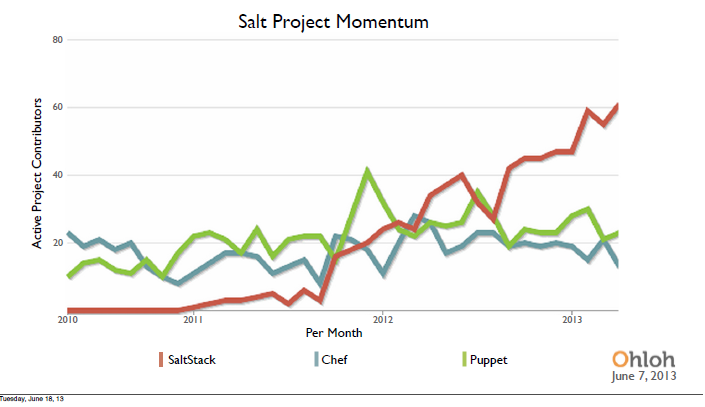
\includegraphics[scale=0.4]{img/salt.png}
	\caption{Porównanie dynamiki rozwoju narzędzi SaltStack, Chef i Puppet na przestrzeni lat 2010-2013\cite{virtualization}}
	\label{salt:chart}
\end{figure}

Jednym z najbardziej dynamicznie rozwijanych rozwiązań (Rysunek \ref{salt:chart}) na rynku jest SaltStack Enterprise\cite{saltstack}. Pozwala ono na sprawne zarządzanie infrastrukturą aplikacji oraz efektywne dostarczanie nowych komponentów do środowiska produkcyjnego. Poza zarządzaniem tradycyjnymi serwerami, SaltStack umożliwa integrację z chmurą i utworzenie abstrakcyjnej, łatwo zarządzalnej warstwy infrastruktury, którą można elastycznie dostosować do różnych aplikacji.
Konkurencyjnym rozwiązaniem, które oferuje automatyzację zarządzania konfiguracją jest Puppet \cite{puppet} występujący w wersji darmowej (Open Source) oraz komercyjnej (Enterprise).

W zestawieniu (Tabela \ref{table:salt}) występują dwa kolejne produkty: Chef oraz Ansible. Opracowanie to zostało przygotowane przez redakcję strony Infoworld, w celu porównania narzędzi wspomagających zarządzanie infrastrukturą aplikacji rozproszonych. Poszczególne produkty zostały ocenione w 10-cio stopniowej skali. Przedstawione kategorie dotyczą zarządzania infrastrukturą aplikacji, ale w dużej mierze pokrywają się z zagadnieniami omówionymi w poprzedniej sekcji (zostały rozszerzone o „Interoperacyjność” oraz „Cena/jakość”). 

\newcommand*\rot{\rotatebox{90}}

\begin{table}[h]
\centering 
\caption{Porównanie narzędzi wspomagających zarządzanie infrastukturą aplikacji \cite{infoworld}}
\label{table:salt}
	\begin{tabular}{@{} cl*{7}c @{}}
		& & \multicolumn{7}{c}{Kategoria oceny i jej waga} \\[2ex]
        & & \rot{Skalowalność (20\%)} & \rot{Dostępność (20\%)} & \rot{Wydajność (20\%)} & \rot{Cena/Jakość (10\%)} 
        & \rot{Zarządzanie usługą (20\%)} & \rot{Interoperacyjność (20\%)}& \rot{Ocena końcowa (100\%)}\\
   		\cmidrule[1px]{2-9}
   		& AnsibleWorks Ansible 1.3 & 8.0 & 9.0 & 9.0 & 9.0 & 8.0 & 7.0 & 8.2 \\
   		& Enterprise Chef 11.4 & 9.0 & 9.0 & 8.0 & 9.0 & 7.0 & 8.0 & 8.3 \\
   		& Puppet Enterprise 3.0 & 9.0 & 9.0 & 9.0 & 9.0 & 9.0 & 9.0 & 9.0 \\
   		\rot{\rlap{~Produkt}}
   		& SaltStack Enterprise 0.17.0 & 9.0 & 9.0 & 9.0 & 9.0 & 9.0 & 8.0 & 8.8 \\
        \cmidrule[1px]{2-9} 
	\end{tabular}
\end{table}

Wszystkie wymienione rozwiązania dostarczają podobnej funkcjonalności, przy czym należy zwrócić uwagę na to, że SaltStack i Ansible to elastyczne i dynamicznie rozwijające się produkty, które stosunkowo niedawno weszły na rynek. Pozostałe dwie pozycje z zestawienia, to bardziej dojrzałe rozwiązania, skierowane przede wszystkim do użytkowników korporacyjnych. Wynika z tego wyższe, w przypadku SaltStack i Ansible, ryzyko znaczących aktualizacji, które mogą mogą wymusić zmiany w projekcie, co sprawia, że te produkty są odpowiednie dla bardziej elastycznych klientów.

\section{Narzędzia do tworzenia wyizolowanych środowisk}

Ta grupa narzędzi koncentruje się na tworzeniu wyizolowanych środowisk deweloperskich w oparciu o instrukcje zapisane w pliku konfiguracyjnym. Popularnym narzędziem tego typu jest Vagrant\cite{vagrant}. Idea tego produktu opiera się na rzeniu maszyny wirtualnej, w której następnie osadzane jest prekonfigurowane środowisko. Kolejne kroki procedury tworzenia tego środowiska są opisane w pliku, który zgodnie z wymogami narzędzia musi nosić nazwę „Vagrantfile”. Niestety, wykorzystanie maszyn wirtualnych wiąże się z narzutem wydajnościowym, a także uzależnia dewelopera od zewnętrznego dostawcy technologii VM (w przypadku Vagrant’a jest to VMWare \cite{vagrant}).

\section{Kontenery aplikacyjne}

Idea kontenerów polena na tworzeniu ``opakowań'' dla aplikacji, które przechowują:

\begin{itemize}
\item kod programu,
\item run time,
\item narzędzia systemowe,
\item biblioteki,
\end{itemize}
niezbędne do poprawnego działania systemu. Jest to ewolucja w stosunku do narzędzi typu Vagrant – kontenery współdzielą ze sobą jądro systemu operacyjnego oraz jego zasoby, natomiast zapewniają izolację na poziomie procesów. Warto zwrócić uwagę na fakt, że jest to technologia oparta na otwartych standardach platformy Linux, na której koncepcja izolacji procesów i ich środowiska jest obecna już od jakiegoś czasu. Kontenery mają za zadanie przede wszystkim zapewnić izolację aplikacji oraz spójność jej środowiska. Adresuje to przytaczane wcześniej problemy, z którymi muszą się mierzyć deweloperzy aplikacji rozproszonych, z naciskiem na redukcję ryzyka wystąpienia konfliktu pomiędzy wykorzystanymi technologiami, braku koherencji środowisk: deweloperskiego, testowego i produkcyjnego, a także trudności z wdrażaniem nowych deweloperów do projektu.

\subsection{Kontenery a maszyny wirtualne}

Główny mechanizm obu rozwiązań jest bliźniaczo podobny (\ref{fig:vm2docker}) – różnica w przypadku kontenerów polega na współdzieleniu przez nie jądra systemu operacyjnego i jego zasobów, dzięki czemu udało się ograniczyć znaczny narzut wydajnościowy jakim obarczone są maszyny wirtualne \cite{infoworld, vagrant, docker}.

\begin{figure}[h]
\centering
\begin{subfigure}{.5\textwidth}
  \centering
  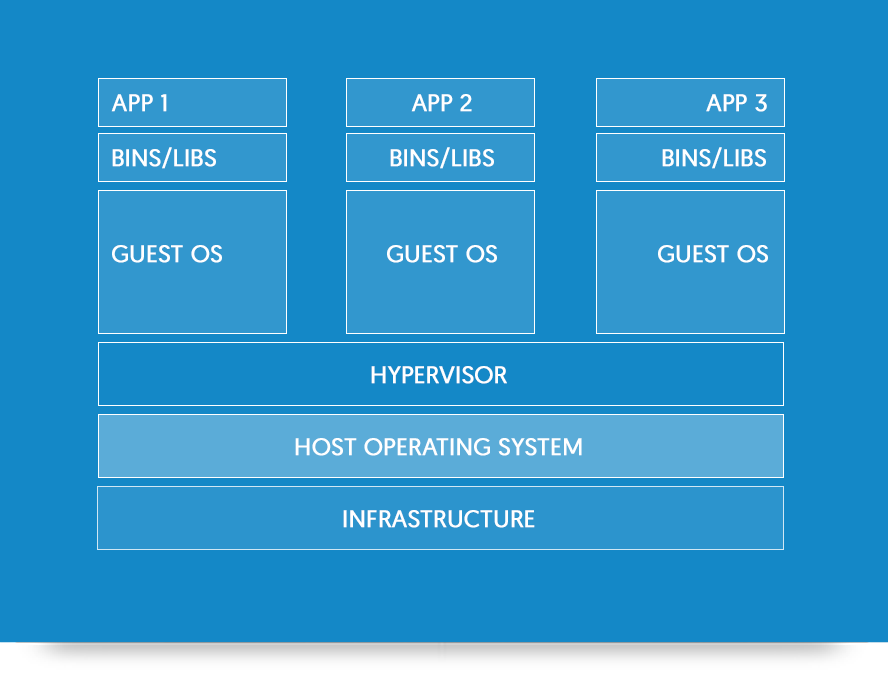
\includegraphics[width=.8\linewidth]{img/vm.png}
  \caption{Architektura maszyny wirtualnej}
  \label{fig:vm}
\end{subfigure}%
\begin{subfigure}{.5\textwidth}
  \centering
  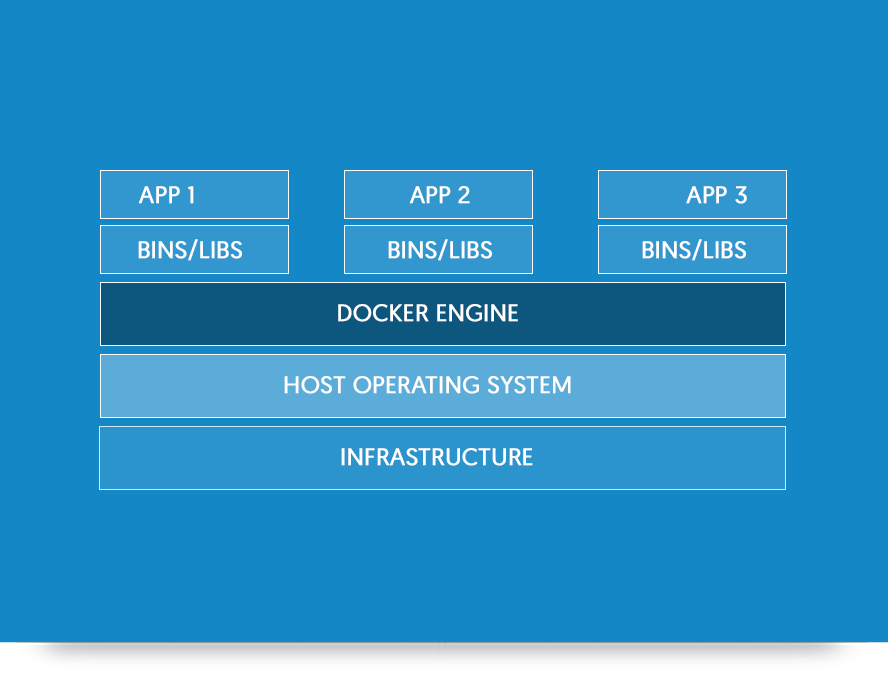
\includegraphics[width=.8\linewidth]{img/docker.png}
  \caption{Architektura kontenera}
  \label{fig:docker}
\end{subfigure}
\caption{Porównanie architetury maszyny wirtualnej i kontenera}
\label{fig:vm2docker}
\end{figure}

\begin{table}[h]
\centering 
\caption{Porównanie kontenerów i maszyn wirtualnych na przykładzie Dockera i Vagranta \cite{docker, vagrant}}
\label{table:vm2docker}
	\begin{tabular}{|p{5cm}|c|c|}
		\hline
		Cecha & Docker & Vagrant \\
		\hline
		Wirtualizacja & Linux Container & VM \\
		\hline
		Czas uruchomienia & Sekundy & Minuty \\
		\hline
		Zarządzanie konfuguracją & Nie & Tak \\
		\hline
		Czas budowania & Pojedyncze minuty & > 10 Minut \\
		\hline
		Maksymalna liczba aplikacji uruchomionych w obrębie jednego serwera & > 50 & < 10 \\
		\hline
		Orkiestracja & CoreOS, Mesos, Kubernetes & Terraform \\
		\hline
		Publiczne repozytorium & DockerHub & VagrantCloud \\
		\hline
		Rozmiar & 100MB+ & 1GB+\\
		\hline
	\end{tabular}
\end{table}

Tabela \ref{table:vm2docker} przedstawia krótkie porównanie obu technologii stworzone na podstawie ich dokumentacji. Na szczególną uwagę zasługują diametralne różnice dotyczące zapotrzebowania na przestrzeń dyskową oraz czasu uruchomienia - są one przynajmniej jednego rzędu wielkości.

\subsection{Docker jako implementacja koncepcji kontenerów}

Początkowo Docker był warstwową implementacją Linux Containers. Narzędzie bardzo szybko zyskało rzeszę zwolenników i wyróżniało się na konferencjach technologicznych, dzięki czemu zdobyło inwestorów aktywnie wspierających jego rozwój. Wynikiem tej współpracy jest cały wachlarz narzędzi udostępnianych deweloperom:

\begin{itemize}
\item Docker Engine - pierwotny produkt firmy, pozwalający na tworzenie kontenerów;
\item Docker Machine - pozwala na tworzenie hostów wyposażonych w technologię Docker na pojedynczych maszynach oraz w chmurze;
\item Docker Compose - pozwala na definiowanie i uruchamianie aplikacji składających się z wielu kontenerów;
\item Docker Swarm - pozwala na tworzenie klastrów dedykowanych rozwiązaniu Docker. Wiele niezależnych maszyn jest łączonych w pojedynczego wirtualnego hosta, który jest transparentny dla koneterów;
\item Docker Registry - pozwala na przechowywanie i dystrybucję obrazów kontenerów;
\item Kitematic - interfejs graficzny umożliwiający zarządzanie kontenerami.
\end{itemize}

\subsection{Integracja maszyn wirtualnych i kontenerów}

Istnieje możliwość połączenia obu rozwiązań w uzasadnionych przypadkach, np. w sytuacji, kiedy maszyna wirtualna odpowiada za konfigurację i uruchomienie samego środowiska, wewnątrz którego włączane są następnie konkretne kontenery aplikacyjne. Rysunek \ref{integrateVagrantDocker} prezentuje przykład, w którym Vagrant zarządza tworzeniem maszyny wirtualnej, na której uruchamiany jest Docker zarządzający poszczególnymi komponentami aplikacji.

\begin{figure}[h] \centering %H if want to get it exaclty here
	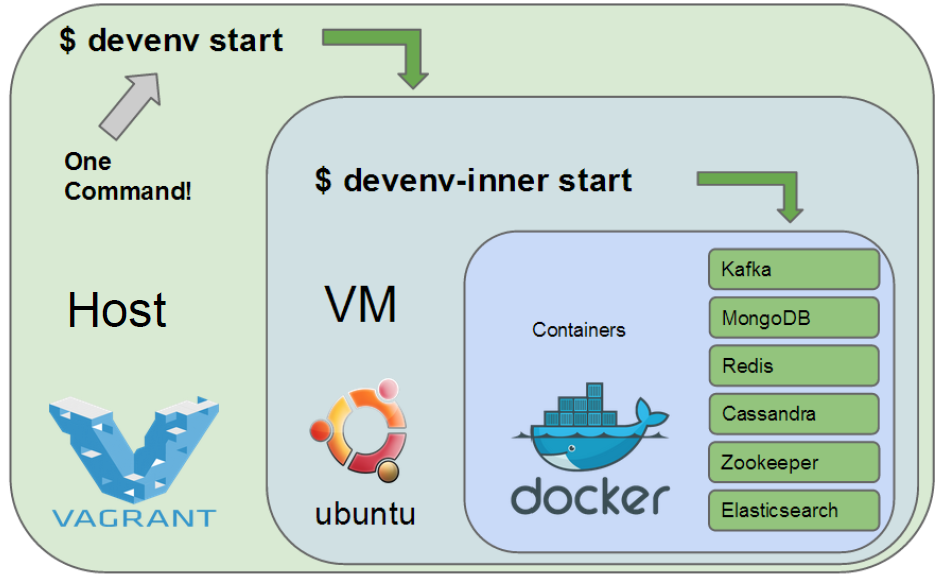
\includegraphics[scale=0.4]{img/integratevagrantdocker.png}
	\caption{Integracja maszyn wirtualnych i kontenerów \cite{ociweb}}
	\label{integrateVagrantDocker}
\end{figure}

\subsection{Struktura obrazów Dockera}

Kontenery są przechowywane w postaci obrazów. Tworzenie nowych obrazów jest możliwe poprzez edycję, czyli dodawanie kolejnych warstw do już istniejących obrazów lub z wykorzystaniem Dockerfile – metoda analogiczna do tworzenia maszyn wirtualnych w oparciu o Vagrantfile, rozszerzona o pobieranie kodu aplikacji bezpośrednio z repozytorium, który jest następnie kompilowany w obrębie kontenera. Każdy krok opisany w Dockerfile, w tym pobranie i kompilacja kodu, tworzy nową warstwę, która rozszerza istniejący obraz. Ponadto istnieje możliwość tworzenia połączeń między kontenerami, co ułatwia korzystanie z poszczególnych modułów aplikacji (np. bazy danych). Docker pozwala na współdzielenie zasobów ze światem zewnętrznym, dzięki czemu aplikacje mogą przetwarzać pliki udostępniane również innym systemom.

\section{CoreOS}

Podstawową różnicą pomiędzy CoreOS \ref{coreOS}, a innymi systemami operacyjnymi z rodziny UNIX jest to, że instalację pakietów oprogramowania zastąpiono włączaniem kolejnych kontenerów Docker do ekosystemu systemu operacyjnego. CoreOS składa się z trzech głównych komponentów:

\begin{itemize}
\item narzędzia odkrywania usług etcd,
\item silnika Docker,
\item manager'a systemu i usług dla środowiska
Linux systemd.
\end{itemize}

\begin{figure}[h] \centering %H if want to get it exaclty here
	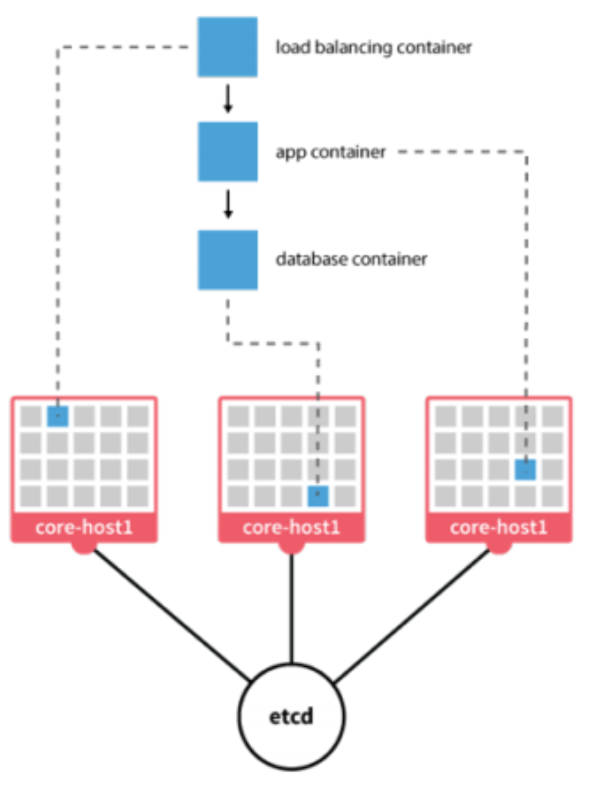
\includegraphics{img/coreOS.png}
	\caption{Struktura CoreOS\cite{coreOS}}
	\label{coreOS}
\end{figure}

Rysunek \ref{coreOS} przedstawia architekturę, w której kontenery z poszczególnymi modułami aplikacji zostają umieszczone na różnych maszynach w oparciu o informacje zawarte w plikach systemd. Nawiązanie komunikacji pomiędzy komponentami następuje z wykorzystaniem narzędzia etcd.

\subsection{Odkrywanie usług z wykorzystaniem etcd}

CoreOS został stworzony i zaprojektowany z myślą o rozproszonych systemach informa- tycznych, co zrodziło zapotrzebowanie dyna- micznego odkrywania usług wystawianych przez aplikacje. Każdy z hostów udostępnia port usłudze etcd, która jest stosowana nie tylko do odkrywania usług, ale również odczytu i zapisu danych konfiguracyjnych. Zamiast umieszczać w kodzie informację o topologii aplikacji (np. bazie danych) wystarczy, że wykorzystamy etcd do ustalenia szczegółów wymaganego połączenia. Moduł aplikacji rejestruje się w usludze etcd podając klucz, który następnie będzie używany przy mapowaniu zapytań typu REST, oraz przypisaną mu wartość (np. klucz „/database” i odpowiadający mu adres bazy danych). Następnie zachodzi replikacja danych konfiguracyjnych w obrębie klastra, dzięki czemu aplikacje uruchomine na różnych maszynach mają lokalny dostęp do aktualnych informacji.

\subsection{Tworzenie klastra kontenerów w oparciu o pliki systemd i narzędzie Fleet}

Pliki systemd opisują poszczególne jednostki wchodzące w skład klastra. W tych opisach można zawrzeć deklracje konfliktów pomiędzy poszczególnymi modułami aplikacji, a także preferencje co do rozmieszczenia tych modułów (np. wymaganie, aby kontener zawierający bazę danych został umieszczony na innej maszynie niż ta, która przechowuje jej backup). Następnie w oparciu o informacje zawarte w plikach systemd następuje przydzielenie kontenerów do konkretnych fizycznych maszyn. Ma to zastosowanie w przypadku usług, które muszą się charakteryzować wysoką dostępnością. W takim wypadku kontenery przechowujące aplikację zostaną umieszczone na niezależnych maszynach, które dodatkowo mogą znajdować się w różnych regionach.